% main.tex - a driver for your Stata Journal insert
%
% This file should only be changed according to the AUTHOR notes below.
%
% The Stata Press document class
\documentclass[bib]{statapress}

% Page dimensions
\usepackage[crop,newcenter,frame]{pagedims}

% The Stata Journal styles
\usepackage{sj}

% Encapsulated PostScript figures
\usepackage{epsfig}

% Stata Log listings and useful macros
\usepackage{stata}

% Shadow package to render technical note figure
\usepackage{shadow}

% Author packages
\usepackage{amsmath}
\usepackage{tikz, tabularx, booktabs, ulem}
\usetikzlibrary{arrows, fit,positioning}


% EDITORS: volume number, issue number, month, and year
\sjsetissue{$vv$}{$ii$}{$mm$}{$yyyy$}

\def\unix1{Intel Xeon X470 (hexadeca-core)}
\def\windows1{Intel i3 2120 (dual-core)}

\begin{document}

% AUTHOR:  Change "readme" to your insert's file name.
\inserttype[st0001]{article}
\author{G. Vega Yon}{%
  George G. Vega Yon\\ g.vegayon@gmail.com
}
\title[parallel]{PARALLEL: Stata Module for Parallel Computing}

\maketitle

\begin{abstract}
With a multicore CPU computer, Stata users can achieve a substantial performance improvement using parallel: a module for parallel computing by means of shell scripting. Parallel can launch up as many Stata executables in batch mode as cores the CPU has to accelerate computations. By splitting the dataset, or repeated loading, into cluster parallel will repeat a task simultaneously over each core, which results in an efficiency improvement proportional to the number of CPU cores. Parallel delivers ``kitchen sink'' parallel computing to the data scientist. In this article we present its main features and show empirical applications using the command.

\keywords{\inserttag, parallel computing, simulations, high performance computing}
\end{abstract}

Parallel computing is becoming reachable each day. Most modern computers processors consists in at least two cores. Frequently associated with \textit{multitasking} users, many single applications can, and do, take advantage of having more than one processor.

A very close example, StataMP version. Making use of multi-processor computers, StataMP has managed to deliver out-of-the-box parallel computing capabilities to Stata without the user having to hold technical knowledge on parallel computing. That is how with StataMP users can do faster linear algebra, faster OLS estimation, and faster data management in general. Nevertheless, while quite a big advance, there is still space to improve its parallel computing capabilities.

For a start, the Multiprocessor version of Stata will not improve neither simulations or bootstrapping estimators \textit{per se}, since the parallelization required to increase its performance relies on task and data-parallelization, this is, a higher (as in more simple, but specific) sort of parallelization. This is how \textit{parallel} is originated.

\section{Features}

The latest version of parallel includes several built-in commands to take advantage of multicore processors, in particular, appending several datasets, running simulations, bootstrapping estimation, and embarrassingly parallel computing. These are described as follows:

\subsection{appending datasets}

\begin{verbatim}
parallel append [file(s)] , do(cmd|dofile) [in(in) if(if) expression(expand expression (see details)) processors(#) programs(namelist)
randtype(current|datetime|random.org) timeout(#)]

\end{verbatim}

\subsection{simulations}

\subsection{bootstrapping estimation}

\subsection{embarrassingly parallel computing}


\section{Extended example: Multiple imputation}

\section{Introduction}

Multicore CPUs are standard in today’s personal computer industry, and potentially move productivity upward for multi-tasking users. Several mathematical and statistical packages make good use of multicore CPUs, for example, MATLAB provides its own Parallel Computing Toolbox\footnote{\url{http://www.mathworks.com/products/parallel-computing/}} which makes it possible to implement parallel computing methods through a multicore computer, GPUs and computer clusters. Alternatively, the GNU open-source R software does offer several packages to implement parallel computing algorithms such as ``parallel'' and ``snow''\footnote{For more details see CRAN Task View on High-Performance and Parallel Computing With R \url{http://cran.r-project.org/web/views/HighPerformanceComputing.html}}. 
With its multiprocessor edition, Stata/MP, Stata Corp. offers bit level parallellization that makes it possible to achieve up to (or greater than) constant scale speed improvements (\citet{stata2010}). However, besides of the fact that users must acquire special editions, some times bit level parellelization is not enough.

By using data or task parallelism, the module parallel allows the Stata user to drastically decrease the time required to complete repetitive computational problems. Parallel makes it possible to implement algorithms characterized by a large number of calculations or, in the case of Stata, code interpretation such as control-flow statements, like loops or simulation models.

\section{Parallelization of Stata}

To speedup computations, a dataset can be split and distributed over a given number of clusters and in so doing implement a data parallelism algorithm. Figure \ref{fig:howworks} illustrates this below the first block when parallel splits the dataset into n clusters.\footnote{Or not, considering that the command also allows to work without data as it the user can also take advantage from just calling n Stata batch mode instances.} Parallel starts n new independent Stata instances in batch mode by which the same task is simultaneously executed. By default, all loaded instance’s globals and programs are passed through. Optionally, mata programs (as mata libs) and objects are passed through as well. After every cluster stops, the result datasets are appended and returned to the current Stata instance without modifying other elements.

\begin{figure}[tb]
\caption{How parallel works\label{fig:howworks}}
\bigskip
\centering
\scalebox{1}{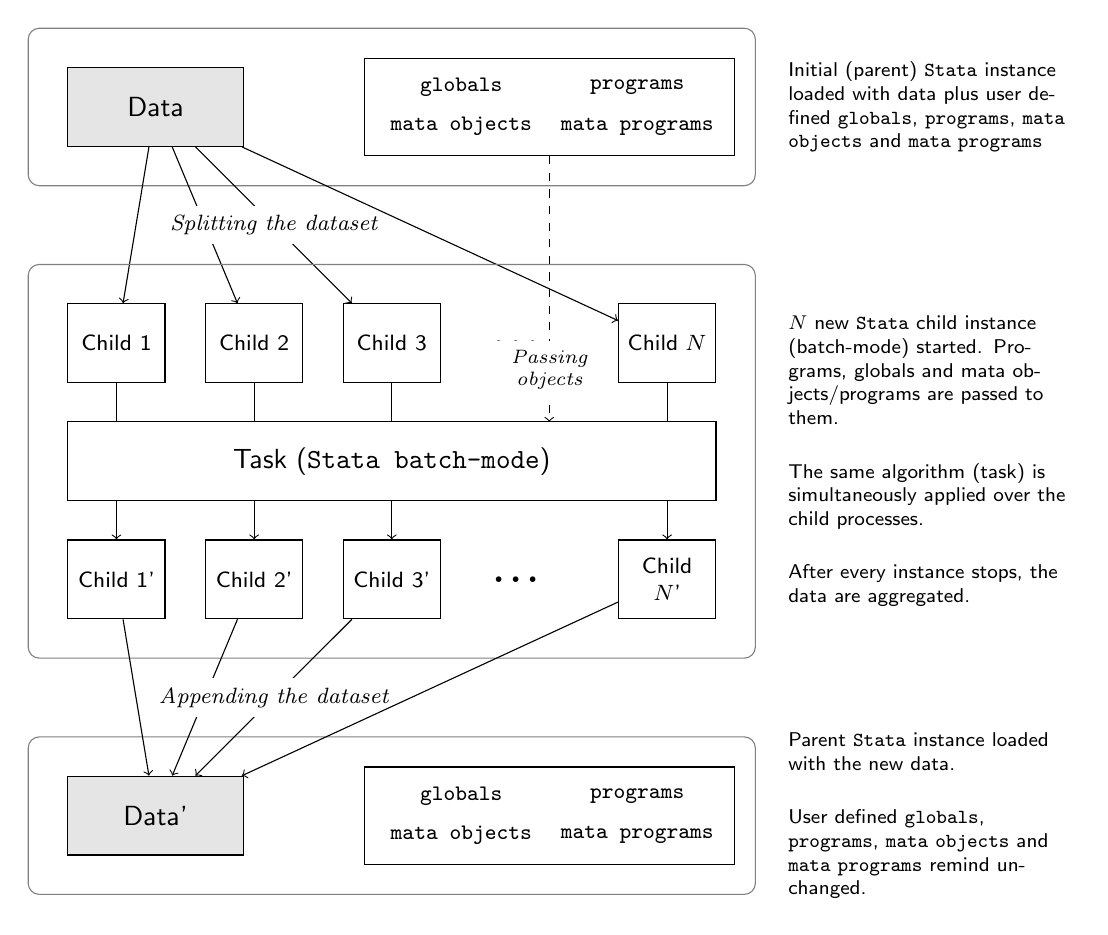
\begin{tikzpicture}[
	every node/.style={node distance=.5cm and .5cm, font=\sffamily}, 
	datablock/.style={rectangle, draw, fill=black!10, text width=2cm, minimum height=1cm, text badly centered},
	cluster/.style={rectangle, draw,text width=1cm, text badly centered, minimum height=1cm, font=\footnotesize\sffamily},
	explain/.style={rectangle, text width=4cm, align=left, font=\footnotesize\sffamily, node distance=.3, scale=.9}
	] 
	
\node [rectangle, draw=gray, text width=9cm, minimum height=2cm, rounded corners] (Stata instance0) at (0,0) {};

% Original data
\node [datablock] (data) at (-3,0) {Data};
\matrix [
	draw=black,
	nodes={
		rectangle, text width=2cm, minimum height=.5cm, 
		scale=1,
		font=\tt\footnotesize, text badly centered}, column sep=0, row sep=0
	] (others) at (2,0) {
	\node {globals};& \node {programs}; \\
	\node {mata objects}; & \node {mata programs}; \\
};

% Data clusters
\node [cluster] (cluster3) at (0,-3) {Child 3};
\node [cluster, left=of cluster3] (cluster2) {Child 2};
\node [cluster, left=of cluster2] (cluster1) {Child 1};
\node [rectangle, right=of cluster3, text width=1cm, font=\Huge] (threepoints) {...};
\node [cluster, right=of threepoints,text badly centered] (clustern) {Child $N$};

% Splitting
\draw[->] (data) -- (cluster1);
\draw[->] (data) -- (cluster2);
\draw[->] (data) -- node [fill=white, font=\footnotesize\it] {Splitting the dataset} (cluster3);
\draw[->] (data) -- (clustern);

\draw[->, dashed] (others) -- node [fill=white, font=\scriptsize\it, below=.65cm, text width=1.2cm, minimum height=.7cm,text badly centered] {Passing objects} (2,-4);

% Procesed clusters
\node [cluster] (cluster3p) at (0,-6) {Child 3'};
\node [cluster, left=of cluster3p] (cluster2p) {Child 2'};
\node [cluster, left=of cluster2p] (cluster1p) {Child 1'};
\node [rectangle, right=of cluster3p, text width=1cm, font=\Huge] (threepointsp) {...};
\node [cluster, right=of threepointsp,text badly centered] (clusternp) {Child $N$'};

\draw[->] (cluster1) -- (cluster1p);
\draw[->] (cluster2) -- (cluster2p);
\draw[->] (cluster3) -- (cluster3p);
\draw[->] (clustern) -- (clusternp);

% Task
\node [rectangle, draw=gray, text width=9cm, minimum height=5cm, rounded corners] (Stata batch) at (0,-4.5) {};
\node [rectangle, fill=white, draw, text width=8cm, text badly centered,minimum height=1cm] (task) at (0,-4.5) {Task (\texttt{Stata batch-mode})};

% Result
\node [rectangle, draw=gray, text width=9cm, minimum height=2cm, rounded corners] (Stata instance1) at (0,-9) {};
\node [datablock] (datap) at (-3,-9) {Data'};
\matrix [
	draw=black,
	nodes={
		rectangle, text width=2cm, minimum height=.5cm, 
		scale=1,
		font=\tt\footnotesize, text badly centered}, column sep=0, row sep=0
	] (othersp) at (2,-9) {
	\node {globals};& \node {programs}; \\
	\node {mata objects}; & \node {mata programs}; \\
};

\draw[->] (cluster1p) -- (datap);
\draw[->] (cluster2p) -- (datap);
\draw[->] (cluster3p) -- node [fill=white, font=\footnotesize\it] {Appending the dataset} (datap);
\draw[->] (clusternp) -- (datap);

% Text
\node [explain, right=of Stata instance0] {Initial (parent) {\tt Stata} instance loaded with data plus user defined {\tt globals}, {\tt programs}, {\tt mata objects} and {\tt mata programs}};

\node [explain, right=of Stata batch] {$N$ new {\tt Stata} child instance (batch-mode) started. Programs, globals and mata objects/programs are passed to them.\\\bigskip The same algorithm (task) is simultaneously applied over the child processes.\\\bigskip After every instance stops, the data are aggregated.};

\node [explain, right=of Stata instance1] {Parent {\tt Stata} instance loaded with the new data.\\\bigskip User defined {\tt globals}, {\tt programs}, {\tt mata objects} and {\tt mata programs} remind unchanged.};

\end{tikzpicture}}
\end{figure}

Parallel is especially helpful in performance a series of computations on the same data sets but with different random samples. Example 5.3 shows how to assess possible sample bias within a cohort using parallel.

\pagebreak

\section{When to use parallel}

Problems that are particularly suitable for data parallelization are:

\begin{itemize}
\item {\bf Control flow statement} Mainly loops. Most loops can be parallelized as these do not require all observations to computer with. Like serial replacing (from observation to observation), loops are a suitable task to parallel computing. In the case that a loop needs to compute with clustered data (loops within individuals in a panel dataset), Stata users can ask parallel to avoid splitting clusters. Example 5.1 shows this.
\item {\bf Clustered computations} Such as an byable egen. Clustered egen can be parallelized without any problem as parallel can avoid splitting clusters. Stata users only have to declare it using the option by().
\item {\bf Bootstrapping} Since a bootstrapping process does not requires to work with all the generated data until the end of it, it is perfect to be computed in parallel process. Parallel allows to run simultaneously random data generation processes using different seeds for each independent computational procedure with reproducible results.
\item {\bf Monte Carlo Simulations} Example 5.2
\item {\bf Reshaping large datasets} Better than Stata/MP, parallel has shown to efficiently reshape large administrative datasets faster. Even though speed gains are not that of the examples showed in this article, parallel reaches speed improvements where Stata/MP does not. 
\item {\bf Cohort sampling tasks like bias testing} Example 5.3
\end{itemize}

\section{Syntax}

\noindent Setting the number of clusters (data blocks)

\begin{stsyntax}
parallel setclusters \#
	\optional{,
	\underbar{f}orce
	\underbar{s}tatadir(\ststring)
	}
\end{stsyntax}

\noindent Parallelizing a do-file

\begin{stsyntax}
parallel do {\it filename}
	\optional{, 
	by(\varlist) 
	\underbar{f}orce 
	\underbar{k}eep 
	\underbar{keepl}ast 
	\underbar{p}rograms 
	\underbar{m}ata
	\underbar{nog}lobal
	\underbar{s}eeds({\it numlist})
	\underbar{nod}ata
	\underbar{r}andtype({\it datetime$|$random.org})
	\underbar{t}imeout({\it integer})
	\underbar{pr}ocessors({\it integer})}
\end{stsyntax}

\noindent Parallelizing a Stata command

\begin{stsyntax}
parallel
	\optional{, 
	by(\varlist) 
	\underbar{f}orce 
	\underbar{k}eep 
	\underbar{keepl}ast 
	\underbar{p}rograms 
	\underbar{m}ata
	\underbar{nog}lobal
	\underbar{s}eeds({\it numlist})
	\underbar{nod}ata
	\underbar{r}andtype({\it datetime$|$random.org})
	\underbar{t}imeout({\it integer})
	\underbar{pr}ocessors({\it integer})}: {\it stata\_cmd}
\end{stsyntax}

\noindent Removing auxiliary files

\begin{stsyntax}
parallel clean 
	\optional{, 
	\underbar{e}vent({\it pll\_id})
	\underbar{a}ll
	}
\end{stsyntax}

\subsection{Options}

\noindent Setting the number of clusters (data blocks)

\hangpara
{\tt force} In order to protect the users' computers, setting more than 8 clusters it is not permitted (see the WARNING in description). With this option the user can skip this restriction.

\hangpara
{\tt statadir} File path. parallel tries to automatically identify Stata's exe path. By using this option you will override this and force parallel to use a specific path of stata.exe.

\noindent Byable parallelization

\hangpara
{\tt by} Varlist. Tells the command through which observations the current dataset can be splitted, avoiding stories splitting over two or more clusters (for example).

\hangpara
{\tt force} When using by, parallel checks whether if the dataset is properly sorted. By using force the command skips this check.

\noindent Keeping auxiliary files

\hangpara
{\tt keep} Keeps auxiliary files generated by parallel.

\hangpara
{\tt keeplast} Keeps auxiliary files and remove those last time saved during the current session.

\noindent Passing Stata/Mata objects

\hangpara
{\tt programs} In the case of having temporal programs loaded in the session, using this option parallel passes them to the clusters.

\hangpara
{\tt mata} If the algorithm needs to use mata objects, this option allows to pass to each cluster every mata object loaded in the current session (including functions).

\hangpara
{\tt noglobal} By default parallel takes into account every global macro loaded in the session. If the user needs to not include globals in clusters, he should use this option.

\noindent Simulation options

\hangpara
{\tt seeds}  Numlist. With this option the user can pass an specific seed to be used within each cluster.

\hangpara
{\tt nodata} Tells parallel that there is no data loaded and thus should not try to split or append anything.

\hangpara
{\tt randtype} String. Tells parallel whether to use the current seed to generate the seeds for each clusters (default option) or use the current datetime -datetime- or random.org API -random.org- (please read the Description section).

\noindent Removing auxiliary files

\hangpara
{\tt event} Integer. Specifies which executed (and stored) event's files should be removed.

\hangpara
{\tt all} Tells parallel to remove every remanent auxiliary files generated by it in the current directory.

\noindent Other options

\hangpara
{\tt timeout} Integer.If a cluster hasn't start, how much time in seconds does parallel has to wait until assume that there was a connection error and thus the child process (cluster) won't start. Default value is 60.

\hangpara
{\tt processors} Integer. If running on StataMP, sets the number of processors each cluster should use. Default value is 0 (do nothing).



\section{Examples}

Others examples are included in the Stata Help file of the command.

\subsection{Serial replacing}

This first test consists on, after a generation of N pseudo-random values, using Stata's {\tt rnormal()} function, replacing each and every one of the observations in a serial way (loop) starting from $1$ to $N$. The observation's variable was replaced using the PDF of the normal distribution

\begin{equation*}
f(x) = \frac{1}{\sqrt{2 \pi}}e^{\frac{-x^2}{2}}
\end{equation*}

The code to be parallelized is

% % % % 
(INSERT CODE HERE)

\noindent which is contained inside a do-file named ``myloop.do'', and can be executed through four clusters with parallel as it follows

(INSERT CODE HERE)

This algorithm was repeated over $N \in \{10000;100000;1000000;10000000\}$

\begin{table}[!h]
\centering
\caption{Serial replacing using a loop on a Linux Server (16 clusters)}
\begin{tabular}{l*{3}{c}}\toprule
& 100.000 &         1.000.000 &       10.000.000 \\ \midrule
CPU &     1.43 &     16.94 &    144.68 \\
Total &     0.34 &      3.20 &     12.49 \\
\hspace{2mm} Setup &     0.00 &      0.00 &      0.00 \\
\hspace{2mm} Compute &     0.32 &      3.07 &     11.54 \\
\hspace{2mm} Finish &     0.02 &      0.12 &      0.95 \\
\midrule Ratio (compute) &     4.50 &      5.51 &     12.53 \\
Ratio (total) &     4.22 (26\%) &      5.30 (30\%) &     11.58 (72\%) \\
\bottomrule
\multicolumn{4}{l}{\footnotesize Tested on a \unix1 machine}
\end{tabular}

\endinput
\end{table}

\subsection{Extended Example 1: Montecarlo Simulation}

In \citet{baum2007} a simple Monte Carlo experiment is perform which simulates the performance of a estimator of sample mean, bar x, in a context of heteroskedasticity.

The model to be

\begin{equation}
y_i = \mu + \epsilon_i \sim N(0,\sigma^2)
\end{equation}

Let $\epsilon$ be a $N(0,1)$ variable multiplied by a factor $cz_i$, where $z_i$ varies over $i$. We will vary parameter $c$ between 0.1 and 1.0 and determine its effect on the point and interval estimates of $\mu$; as a comparison, we will compute a second random variable which is homoskedastic, with the scale factor equalling $c\bar z$.

From web dataset {\tt census2} the variables {\tt age}, {\tt region} (which can be 1, 2, 3 or 4) and the mean of {\tt region} are used as $\mu$, $z_i$ and $\bar z$ respectively.

The simulation program, stored in ``mcsimul1.ado'', is defined as

(INSERT CODE HERE)

In what is next, the do-file that runs the simulation, stored as ``montecarlo.do'', it is compound of two parts: (a) setting the iteration range by which $c$ is going to vary, and (b) looping over the selected range. For the first part the do-file uses the local macro {\tt pll\_instance} which is the numer of the parallel stata instance running, thus there are as many as clusters have been declared, number available with the global macro {\tt PLL\_CLUSTERS}. This way, if the macro {\tt PLL\_CLUSTERS} equals two and the macro {\tt pll\_instance} equals une, then the range will be defined from one to five\footnote{Note that if the local macro {\tt pll\_id}, which contains a special random number that identifies an specific {\tt parallel} run (more details in its help file), length is zero it means that the do-file is not running in parallel mode, thus it is been executed in a serial way where the loop range starts from one to ten.}.
\bigskip

(INSERT CODE HERE)

\noindent This do-file will be executed from stata using {\tt parallel do} syntax. As there is no need of splitting any dataset (these are loaded every time that the main {\tt loop\_simul.do}'s loop runs), we add the option {\tt nodata}. This way the main do-file will look like this
Finally, the do-file from which parallel runs the simulation

(INSERT CODE HERE)

By this {\tt parallel} will start, in this case, five new independent stata instances, each one looping over the ranges 1/2, 3/4, 5/6, 7/8 and 9/10 respectively.

Most of the code has been exactly copied with the exception of the addition of a new code line {\tt set seed}. In order to be able to compare both serial and parallel implementations of the algorithm it was necessary to set a particular seed for each loop, inside ``montecarlo.do'' right before {\tt simulate} command.

\begin{table}[!h]
\centering
\caption{Monte Carlo Experiment on a Windows Machine (4 clusters)}
\begin{tabular}{l*{2}{c}}\toprule
& 2 &               4 \\ \midrule
CPU &   111.49 &    114.13 \\
Total &    58.02 &     37.48 \\
\hspace{2mm} Setup &     0.00 &      0.00 \\
\hspace{2mm} Compute &    58.02 &     37.48 \\
\hspace{2mm} Finish &     0.00 &      0.00 \\
\midrule Ratio (compute) &     1.92 &      3.04 \\
Ratio (total) &     1.92 (96\%)&      3.04 (76\%)\\
\bottomrule
\multicolumn{3}{l}{\footnotesize Tested on a \windows1 machine}
\end{tabular}

\endinput
\end{table}

\begin{table}[!h]
\centering
\caption{Monte Carlo Experiment on a Linux Server (16 clusters)}
\begin{tabular}{l*{4}{c}}\toprule
& 2 &               4 &               8 &              16 \\ \midrule
CPU &   164.79 &    164.04 &    162.84 &    163.89 \\
Total &    69.85 &     34.28 &     19.00 &     10.78 \\
\hspace{2mm} Setup &     0.00 &      0.00 &      0.00 &      0.00 \\
\hspace{2mm} Compute &    69.85 &     34.28 &     19.00 &     10.78 \\
\hspace{2mm} Finish &     0.00 &      0.00 &      0.00 &      0.00 \\
\midrule Ratio (compute) &     2.36 &      4.78 &      8.57 &     15.21 \\
Ratio (total) &     2.36 (118\%) &      4.78 (120\%)&      8.57 (107\%) &     15.21 (95\%) \\
\bottomrule
\multicolumn{4}{l}{\footnotesize Tested on a \unix1 machine}
\end{tabular}

\endinput
\end{table}


% Bib
\bibliographystyle{sj}
\bibliography{bib}

\end{document}
% END: main.tex
